
\chapter{Comparación y análisis de las librerías}\label{desarrollo}
\renewcommand{\thefootnote}{\arabic{footnote}}

De cara a analizar las librerías se desarrollará una aplicación con cada una de ellas. La aplicación consistirá en instanciar un dragón obtenido de la Asset Store de Unity \cite{AssetStore}.\\

Los test se desarrollarán en dos condiciones lumínicas diferentes, luz mínima y ambiental.
Como luz mínima se considerará una sala de unos 20m\textsuperscript{2} únicamente iluminada por un haz de luz perteneciente a una habitación contigua. En cambio, como luz ambiente se considerará esta misma sala iluminada por cuatro ventanas a la luz de la tarde.\\

El dispositivo que se utilizará para realizar todas las pruebas será el Pocophone F1. A excepción de las librerías ARKit y Vuforia, que serán probadas con un Iphone 8 Plus debido a que el Pocophone F1 no está en la lista de dispositivos soportados en Vuforia Fusion \cite{Vuforia_Devices} y ARKit únicamente soporta dispositivos iOS.\\

Para realizar la evaluación de las capacidades y los límites de cada librería se realizará un test que consistirá en:
\begin{itemize}
\item Instanciar un objeto.
\item Movernos alrededor de dicho objeto, para comprobar la estabilidad del punto de anclaje.
\item Realizar movimientos bruscos y veloces en el teléfono para ver si pierde la referencia en algún momento.
\item Sacar al objeto del campo de visión de la cámara y ver cómo reacciona cuando al volver.
\item Alejarnos del objeto y ver hasta que distancia sigue funcionando.
\item Observar la calidad de las texturas.
\item Observar la estimación de luces.

\end{itemize}

Una vez realizadas las pruebas el análisis de las librerías se estructurará en los puntos que se describen a continuación:
\begin{itemize}
\item Calidad de la documentación y primeros pasos: en este punto evaluaremos la dificultad para realizar una aplicación básica con cada librería, desde el momento en el que se descarga el SDK, hasta que se construye la aplicación. 
\item Evaluación de las capacidades de la librería: en este apartado se tendrán en cuenta las funcionalidades, las tecnologías que soporta y el nivel personalización dentro de la aplicación, es decir, hasta que nivel podemos usar la API que nos proporcionan.
\item Conclusiones: gracias al estudio realizado estableceremos unas conclusiones sobre el uso de cada librería y decidiremos si nos facilita el desarrollo de alguna prueba de concepto.
\end{itemize}

Las aplicaciones y desarrollo de las pruebas se encuentran almacenadas en el repositorio: \url{https://github.com/ar-tfg/DemosLibrerias}.\\

Los vídeos de las evaluaciones se encuentran almacenados en la siguiente lista de reproducción de Youtube \url{ https://www.youtube.com/playlist?list=PLqQgTAUiabc8AQrcc48Jdglnytus9IoXe}.



\section{Wikitude}

\subsection{Calidad de la documentación y primeros pasos}
La experiencia al crear una aplicación usando Wikitude es buena. Te guían desde el momento en el que entras a la web para descargar el SDK que necesites, eso sí, hace falta registrarse y descargar una clave de licencia para que funcione la aplicación. Dicha clave hay que introducirla en el componente Wikitude Camera que trae el paquete. Todos estos pasos vienen documentados, para facilitar el proceso de prueba, el paquete incluye varias escenas montadas en las que se pueden probar diferentes tipos de tecnologías. Para hacer funcionar todas las escenas, es necesario que el \textit{Package Name} de la aplicación sea ``com.wikitude.unityexample'', ya que el SDK está protegido de esta manera. La documentación de la API es muy completa y está muy bien estructurada~\cite{WikitudeDoc}.
\subsection{Evaluación de las capacidades de la librería}
\textbf{Condiciones de luz mínimas:}\\
\url{https://youtu.be/_4fLQas1NcM}\\

Consigue instanciar el objeto dentro de un plano y posee buena iluminación. El plano falla cuando empezamos a movernos haciendo un giro de 45º no esperado, si estamos encima del modelo se pierde, si damos la vuelta completa sigue perdido. Necesitamos volver a referenciarlo por que no se recupera. La calidad del modelo y su textura es óptima para las condiciones de luz que posee. Se pierde la referencia fácilmente ante los giros. Cuando se realiza un movimiento de cámara en el que el punto de anclaje sale del campo de visión y más tarde se vuelve a enfocar a él, tarda un segundo en volver a posicionar el plano y su objeto. En esta prueba no hemos conseguido que pierda la referencia por distancia. Hace estimaciones con oclusión desapareciendo con la pared.\\

\textbf{Condiciones de luz ambiente:}\\
\url{https://youtu.be/wlqITlPTz3o}\\

Consigue instanciar el objeto dentro de un plano y posee buena iluminación. El plano falla cuando empezamos a movernos haciendo de nuevo un giro de 45º no esperado, si estamos encima del modelo se pierde pero en este caso se recupera con cierta facilidad. Podemos acercarnos bastante manteniendo el nivel de detalle. La calidad del modelo y su textura es óptima para las condiciones de luz que posee. Se pierde la referencia fácilmente ante los giros. Cuando se realiza un movimiento de cámara en el que el punto de anclaje sale del campo de visión y más tarde se vuelve a enfocar a él, tarda menos de un segundo en volver a posicionar el plano y su objeto. En esta primera prueba no hemos conseguido que pierda la referencia por distancia. Hace estimaciones con oclusión desapareciendo con la pared.

\begin{table}[H]
    \centering
    \begin{tabular}{l c c}
    \toprule
        & Luz Ambiente & Luz Mínimas \\
         \midrule
        Estabilidad del punto de anclaje   &3 &6\\
        
        Estimación y calidad de iluminación  &4 &6 \\
        
        Resistencia a movimientos  &1 &2 \\
        
        Recuperación del ancla  &8 &8 \\
      \bottomrule
    \end{tabular}
    \caption{Análisis Wikitude}
    \label{tab:TWikitude}
\end{table}

\subsection{Conclusiones}
A pesar de ser una de las librerías pioneras en el sector, los resultados obtenidos no son tan buenos frente a sus competidores, por lo menos en lo que a realidad aumentada sin marcadores se refiere. Lo peor de esta librería es la resistencia a movimientos bruscos (y no tan bruscos), desde que el móvil sufre una pequeña agitación, el modelo desaparece, lo cual es desastroso. Por otro lado, hay que destacar es su intento de detectar oclusión, ha sido la única que ha reaccionado cuando hemos cruzado una pared.

\section{ARKit}
\subsection{Calidad de la documentación y primeros pasos}
La documentación de ARKit es muy extensa y detallada y con una comunidad amplia y activa favoreciendo el desarrollo de aplicaciones con esta tecnología. Existe un plugin para Unity que permite el desarrollo en la plataforma.  Para hacer funcionar este SDK es tan sencillo como añadirlo desde el gestor de paquetes de Unity. Este paquete permite partir desde una escena vacía o desde el ejemplo aportado por el SDK, gracias al ejemplo la primera toma de contacto con la librería es bastante accesible. Además la documentación de los primeros pasos es una excelente guía para el conocimiento de la librería y el posterior desarrollo.

\subsection{Evaluación de las capacidades de la librería}

\textbf{Condiciones de luz mínimas:}\\ 
\url{https://youtu.be/uwjq-bF_J4M}\\

Necesita significativamente más luz para reconocer el plano, en parte debido al dispositivo. Para esta prueba tuvimos que aumentar la iluminación de la sala. La estimación de la iluminación es excelente como podemos ver a lo largo de la prueba. Al realizar un movimiento alrededor del modelo no se pierde ni se desestabiliza en ningún momento. Al posicionar el teléfono sobre el modelo sigue estable. Las texturas del modelo se ven de manera nítida y realista. En la prueba de resistencia a movimientos bruscos se desplaza el plano en ocasiones recuperándose en un breve periodo de tiempo (menor a un segundo). Cuando se realiza un movimiento en el que el modelo desaparece del campo de visión este no llega a desaparecer nunca del entorno virtual por lo que al volver a enfocar al punto de anclaje la transición es limpia.\\

\textbf{Condiciones de luz ambiente:}\\
\url{https://youtu.be/zcm59hRtJeQ}\\

Reconoce los planos casi instantáneamente, por lo que nos permite posicionar el objeto sin esperas. La calidad de las texturas son muy buenas y la estimación de luz es impresionante, la luz cambia mientras rodeamos al modelo, estando mas oscuro cuando nos encontramos a contraluz, e iluminado cuando nos situamos entre la luz entrante y el modelo. La estabilidad del objeto es sobresaliente, nos permite rodear el objeto y acercarnos todo lo posible sin que se mueva. La resistencia a movimientos bruscos es grande, situando al modelo siempre en su punto origen. Lo mismo ocurre en la prueba de sacar el punto de anclaje del campo de visión de la cámara, el objeto nunca desaparece, por lo que al volver a enfocar el punto de partida, vemos una transición muy natural.


\begin{table}[H]
    \centering
     \begin{tabular}{l c c}
    \toprule
          & Luz Ambiente & Luz Mínimas \\
        \midrule
        Estabilidad del punto de anclaje   &10 &10\\
        
        Estimación y calidad de iluminación  &9 &10 \\
        
        Resistencia a movimientos  &9 &10 \\
        
        Recuperación del ancla  &10 &10 \\
      \bottomrule
    \end{tabular}
    \caption{Análisis ARKit}
    \label{tab:TARKit}
\end{table}

\subsection{Conclusiones}
Como hemos comprobado anteriormente, en unas condiciones de luz mínimas el trabajo de esta librería ha sido casi excelente. Su único fallo era la resistencia a movimientos bruscos, la cual se arregla cuando las condiciones lumínicas son óptimas, pudiendo disfrutar de una experiencia perfecta. Si ya con la luz mínima era casi perfecta, con unas condiciones buenas de luz, estamos ante una de las mejores opciones a la hora de crear una experiencia de realidad aumentada. Cabe destacar que ARKit sólo está soportado en dispositivos iOS, por lo que se puede controlar mucho más el abanico de dispositivos en el que se va a usar la aplicación, lo cual es útil a la hora de asegurar el correcto funcionamiento de las aplicaciones.

\newpage
\section{ARCore}
\subsection{Calidad de la documentación y primeros pasos}
Hacer funcionar una aplicación con ARCore es tan fácil como descargar el SDK desde su Github oficial~\cite{Github_Google}, añadir una de las escenas de ejemplo a la build y seleccionar dentro de Unity3D la opción de ``Player Settings -> XR Settings -> ARCore Supported''. Para probar la realidad aumentada con ARCore no hace falta registrarse ni obtener ninguna licencia para que funcione, exceptuando el uso de los \textit{Cloud Anchors}, en el siguiente capítulo (\ref{bombARdero}) explicaremos cómo activarlos. La documentación de los pasos a seguir y de la API es bastante completa, además al ser una de las librerías más usadas en la comunidad hay muchos tutoriales de los que puedes aprender. Para facilitar el desarrollo de aplicaciones con ARCore, Google ha desarrollado una aplicación \textit{ARCore Instant Preview}, la cual se engancha vía USB o Wifi con el editor de Unity3D, y permite probar las aplicaciones en el teléfono sin necesidad de construir una aplicación.
\subsection{Evaluación de las capacidades de la librería}
\textbf{Condiciones de luz mínimas:}\\
\url{https://youtu.be/uSRztU8z18U}\\

Necesita más luz que las anteriores librerías para posicionar el objeto, debido a esto tuvimos que iluminar un poco más la sala. La estimación de la iluminación es excelente como podemos ver a lo largo de la prueba. Al realizar un movimiento alrededor del modelo no se pierde ni se desestabiliza en ningún momento. Al posicionar el teléfono sobre el modelo sigue estable. Las texturas del modelo se ven de manera nítida y realista. En la prueba de resistencia a movimientos bruscos no desaparece nunca ni vibra la imagen dando unos resultados óptimos. Cuando se realiza un movimiento en el que el modelo desaparece del campo de visión este no llega a desaparecer nunca del entorno virtual por lo que al volver a enfocar al punto de anclaje la transición es limpia.\\

\textbf{Condiciones de luz ambiente:}\\
 \url{https://youtu.be/PLXAEFJn4rQ}\\

En este caso reconoce los planos al instante gracias a las condiciones lumínicas. La estimación de la iluminación es sorprendente, ya que mientras giramos alrededor del modelo la luz reacciona a nuestros movimientos. Podemos observar que al posicionarnos en contraluz el objeto está menos iluminado que al comienzo de la prueba donde la luz era directa. En el segundo caso creemos que la intensidad de la luz estimada es un poco excesiva. Los movimientos de cámara se mantienen como en la primera prueba teniendo un resultado perfecto.

\begin{table}[H]
    \centering
      \begin{tabular}{l c c}
    \toprule
          & Luz Ambiente & Luz Mínimas \\
         \midrule
        Estabilidad del punto de anclaje   &10 &10\\
        
        Estimación y calidad de iluminación  &8 &9 \\
        
        Resistencia a movimientos  &10 &10 \\
        
        Recuperación del ancla  &10 &10 \\
      \bottomrule
    \end{tabular}
    \caption{Análisis ARCore}
    \label{tab:TARCore}
\end{table}
\subsection{Conclusiones}
Los resultados obtenidos con ARCore han sido magníficos. El único punto flojo es cuando las condiciones de luz son muy bajas, porque no es capaz de detectar la superficie. Quitando esa situación, la experiencia obtenida es muy buena, ya que es muy estable y posee estimación de luz que funciona casi a la perfección, exceptuando ciertos momentos en los que es excesivamente luminosa.\\

La mayor limitación de esta librería es su lista de dispositivos soportados~\cite{ARCoreList}. A pesar de que esta lista va creciendo, aún quedan muchos dispositivos que no están soportados, por lo que el público al que puede llegar una aplicación de realidad aumentada usando ARCore es muy limitado.

\section{Vuforia}
\subsection{Calidad de la documentación y primeros pasos}
Los primeros pasos con esta librería en conjunto con Unity son muy ágiles y accesibles, gracias a una documentación de calidad podemos ser guiados paso a paso para la creación de una nueva experiencia de realidad aumentada. La integración con Unity es muy simple gracias a un paquete que podemos descargar desde el propio editor. Una vez instalado el paquete, los pasos necesarios para crear una aplicación que detecta una superficie, es tan simple como añadir dos objetos proporcionados por Vuforia y el modelo que queremos instanciar a la escena. Para que la aplicación funcione, es necesario registrarse en el portal de desarrollo de Vuforia \cite{Vuforia} y generar una clave de licencia. Dicha clave hay que introducirla en el archivo de configuración que incluye el paquete.
\subsection{Evaluación de las capacidades de la librería}

\textbf{Condiciones de luz mínimas:}\\
\url{https://youtu.be/4Y_Enzrx17w}\\

El nivel de luz de la sala no supone ningún problema para posicionar el modelo. La calidad de las texturas del objeto son malas, además no existe ninguna estimación de iluminación sobre el modelo. El anclaje alrededor del objeto con movimientos suaves es malo ya que se mueve con nosotros. La estabilidad del objeto cuando nos movemos en sus proximidades es mala ya que el objeto cambia de posición a medida que nos acercamos. No conseguimos perder el objeto con la distancia. La capacidad de soportar movimientos bruscos es buena, ya que no pierde la posición del ancla. Al sacarlo del campo de visión lo mantiene en su posición en todo momento.\\

\textbf{Condiciones de luz ambiente:\\}
\url{https://youtu.be/zlUj-jh7Uts}\\

Después de mejorar las condiciones de luz se mantienen los problemas de estimación de luz. La visualización del modelo renderiza las texturas de manera muy pobre siendo muy poco realista. La estabilidad del objeto mejora ya que podemos girar alrededor del objeto sin perder la referencia, permitiéndonos acercarnos en esta ocasión. Se mantiene la capacidad de soportar movimientos bruscos y la robustos en cuanto al campo de visión.

\begin{table}[H]
    \centering
     \begin{tabular}{l c c}
    \toprule
          & Luz Ambiente & Luz Mínimas \\
         \midrule
        Estabilidad del punto de anclaje   & 5 & 7\\
        
        Estimación y calidad de iluminación  &2 &2 \\
        
        Resistencia a movimientos  &10 &10 \\
        
        Recuperación del ancla  &10 &10 \\
      \bottomrule
    \end{tabular}
    \caption{Análisis Vuforia}
    \label{tab:TVuforia}
\end{table}

\subsection{Conclusiones}
Los resultados obtenidos con Vuforia no son los esperados ya que se trata de una de las librerías pioneras en la realidad aumentada con marcadores y su resultado dista mucho de sus competidores. El listado de los dispositivos soportados~\cite{Vuforia_Devices} no tiene mucha coherencia ya que están los últimos dispositivos de las marcas principales del mercado como Apple o Samsung y sin embargo en las demás marcas encontramos productos muy antiguos generando problemática a la hora de cubrir un rango amplio de usuarios. Como punto fuerte podríamos establecer su detallada documentación. Además nos ha gustado mucho el detalle de tener una cuadrícula (100cm x 100cm) de referencia en Unity para poder saber las dimensiones del objeto en la realidad.\\

\section{Kudan}
\subsection{Calidad de la documentación y primeros pasos}
Los primeros pasos con Kudan no son tan gratificantes en comparación a sus competidores. Empezando por la descarga del SDK, ésta ni si quiera se encuentra en la página oficial~\cite{Kudan_Official}, si no que se encuentra en XLSoft~\cite{Kudan}. Una vez metido el SDK en Unity, en las carpetas vienen escenas de ejemplo, en las que podemos ver como se monta una aplicación con Kudan. Para que funcione correctamente, hace falta introducir este \textit{Package Name} ``com.xlsoft.kudanar''~\cite{Kudan_License}. La documentación para los primeros pasos es aceptable, pero sobre el SDK y la API no hay documentación, únicamente los comentarios en los scripts. Una vez instalada la aplicación en el teléfono, no funcionará ya que la aplicación no pide los permisos para usar la cámara, y sin ellos Kudan no puede inicializarse. Para arreglar este error, hace falta añadir en algún script estas líneas de código:\\
\begin{lstlisting}
using UnityEngine.Android;
Permision.RequestUserPermission(Permission.Camera);
\end{lstlisting}

\subsection{Evaluación de las capacidades de la librería}

\textbf{Condiciones de luz mínimas:}\\
\url{https://youtu.be/cLJMyV9bV6s}\\

El nivel de luz de la sala no supone ningún problema para posicionar el modelo. La calidad de las texturas del objeto es mala, además no existe ninguna estimación de iluminación sobre el modelo. El anclaje alrededor del objeto con movimientos suaves es aceptable pero en el momento que nos acercamos se pierde y hay que volver a referenciarlo. La estabilidad del objeto cuando nos movemos en sus proximidades es muy mala, cambiando de tamaño sin sentido aparente. La distancia máxima de captura es de siete metros aproximadamente. La capacidad de soportar movimientos bruscos es mala, pierde totalmente la posición del ancla con resultados incorrectos e incluso a veces pierde la referencia del todo. Al sacarlo del campo de visión no lo posiciona en el mismo punto donde estaba, llegando a perder en ocasiones el punto de referencia.\\

\textbf{Condiciones de luz ambiente:}\\
\url{https://youtu.be/JyjBmQZZ5E4}\\

Gracias a las condiciones de luz la estabilidad del objeto en la escena mejora sustancialmente, pudiendo dar la vuelta casi perfecta al objeto sin problemas, exceptuando la posición cenital que genera desestabilización breve en el objeto. Se mantiene la distancia máxima de siete metros. Además en esta ocasión la resistencia ante movimientos bruscos mejora considerablemente, sin llegar a ser correcta ya que pierde la referencia en una ocasión. En el caso del campo de visión recupera el objeto de manera más rápida sin llegar a volver a posicionar con precisión el objeto.

\begin{table}[H]
    \centering
     \begin{tabular}{l c c}
    \toprule
          & Luz Ambiente & Luz Mínimas \\
         \midrule
        Estabilidad del punto de anclaje   &3 &6\\
        
        Estimación y calidad de iluminación  &0 &0 \\
        
        Resistencia a movimientos  &2 &7 \\
        
        Recuperación del ancla  &3 &6 \\
      \bottomrule
    \end{tabular}
  
    \caption{Análisis Kudan}
    \label{tab:TKudan}
\end{table}
\subsection{Conclusiones}
Los resultados obtenidos con Kudan no son muy buenos, además de que no renderiza la cámara en la aplicación, por lo que se ve con un fondo negro, impidiendo que la experiencia sea tan inmersiva frente a las demás librerías. Los resultados con condiciones de luz mínimas han sido muy malos, y aunque cuando hemos aumentado la cantidad de luz ha mejorado bastante, no llega al nivel de los competidores.



\section{Maxst}
\subsection{Calidad de la documentación y primeros pasos}
Para usar Maxst, hace falta registrarse en su página web~\cite{Maxst}, y acceder a la descarga del SDK. Además, hay que generar una clave de licencia específica para nuestro \textit{Package Name}. La documentación  es buena en ambos casos, en la guía de integración y de la API. Una vez importada la librería en Unity, se puede ver que hay escenas de ejemplo ya hechas, por lo que simplemente hay que añadirlas a la \textit{Build} de la aplicación. Se pueden probar las aplicaciones también desde el editor, usando una cámara que esté conectada al ordenador, el resultado es peor que en un móvil, ya que la cámara no tiene sensores, pero sirve para darnos una idea del tamaño de los objetos. 
\subsection{Evaluación de las capacidades de la librería}
\textbf{Condiciones de luz mínimas:}\\
\url{https://youtu.be/QFX_B8HX1yU}\\

El nivel de luz de la sala no supone ningún problema para posicionar el modelo. La calidad de las texturas del objeto son notables, pero no existe ninguna estimación de iluminación sobre el modelo. El anclaje alrededor del objeto con movimientos suaves es aceptable pero en el momento que nos acercamos se pierde y no se llega a recuperar el punto teniendo que volver a referenciarlo.  No somos capaces de dar la vuelta al modelo completo sin perderlo. No conseguimos perderlo con la distancia. La capacidad de soportar movimientos bruscos es mejorable ya que no desaparece el modelo, pero si pierde su referencia en el espacio moviéndolo a una posición diferente. Al sacarlo del campo de visión no lo posiciona de nuevo en la mayoría de las ocasiones. Sin embargo, cuando consigue mantenerlo, en la mayoría de ocasiones se desplaza del punto correcto y muy rara vez muestra la opción correcta.\\

\textbf{Condiciones de luz ambiente:}\\
\url{https://youtu.be/cspBAaQCfew}\\

La estabilidad ha mejorado notablemente, permitiendo dar la vuelta completa. En ocasiones pierde la referencia y se desplaza el modelo un poco si nos acercamos demasiado. Si se pierde el punto de visión por ejemplo cruzando una pared desaparece el modelo, pero si volvemos al punto de partida es capaz de recuperar la referencia en aproximadamente 7 segundos. La resistencia a los giros bruscos ha mejorado considerablemente llegando a ser casi perfecta, a veces se desplaza en algún fotograma pero se reposiciona rápidamente. Al sacar el modelo del campo de visión de la cámara y luego volver a meterlo rinde mejor con el entorno iluminado, consiguiendo que esté bien posicionado, eso sí, a veces sigue desapareciendo y volviendo a aparecer, impidiendo así una transición limpia.

\begin{table}[H]
    \centering
      \begin{tabular}{l c c}
    \toprule
          & Luz Ambiente & Luz Mínimas \\
         \midrule
        Estabilidad del punto de anclaje   &4 &6\\
        
        Estimación y calidad de iluminación  &1 &1 \\
        
        Resistencia a movimientos  &4 &9 \\
        
        Recuperación del ancla  &3 &7 \\
      \bottomrule
    \end{tabular}
    \caption{Análisis Maxst}
    \label{tab:TMaxst}
\end{table}
\subsection{Conclusiones}
Apenas necesita tiempo para posicionar el ancla, no hay que esperar a que reconozca una superficie plana, pero la estabilidad debe mejorar un poco. A pesar de estar en unas condiciones lumínicas ideales, el modelo a veces se mueve cuando estamos muy cerca e incluso puede llegar a perderse la referencia. Esto es crítico si se quiere desarrollar una aplicación en la que se pueda mover alrededor de un punto, o acercarse mucho a él para poder verlo con detalle. 



\section{8th Wall XR}
\subsection{Calidad de la documentación y primeros pasos}
Para desarrollar aplicaciones de realidad aumentada con 8thWall, es necesario registrarse en su página web~\cite{8thWall}, descargar el SDK, y generar una clave de licencia, que tendremos que especificar en el objeto ``XRAppSettings'' que se encuentra dentro del paquete de Unity3D. Estos pasos vienen bien documentados en la guía que proporcionan, por lo que la calidad de la documentación es buena, también en la parte de la API. Tienen tutoriales subidos en los que enseñan y explican cómo desarollar aplicaciones con su SDK. En los dispositivos que se encuentran en la lista de ARCore~\cite{ARCoreList}, 8thWall usa ARCore para la tecnología de realidad aumentada. Para los que no se encuentran en esa lista, tienen su propia tecnología, que no funciona tan bien pero por lo menos permite cubrir un rango muy amplio de dispositivos soportados. Para facilitar el desarrollo, han creado una aplicación para probar en el móvil desde el editor de Unity3D, llamada \textit{8th Wall XR Remote}, que se puede encontrar en \textit{Google Play}~\cite{8thWallRemote}.

\subsection{Evaluación de las capacidades de la librería}
\textbf{Condiciones de luz mínimas:}\\
\url{https://youtu.be/6edM5PhhXj0}\\

El nivel de luz de la sala supone un problema para posicionar el modelo con lo que aumentamos el nivel de luz. La calidad de las texturas del objeto son buenas, además posee estimación de iluminación sobre el modelo correcta y muy eficaz. El anclaje alrededor del objeto con movimientos suaves es muy buena pudiendo dar una vuelta sin problema y acercarnos para ver el detalle del objeto sin que desaparezca. No conseguimos perderlo con la distancia en ningún momento. La capacidad de soportar movimientos bruscos es muy buena, nunca se pierde y su anclaje sigue en la posición correcta. Al sacarlo del campo de visión lo mantiene creando una transición suave.\\

\textbf{Condiciones de luz ambiente:}\\
\url{https://youtu.be/5TBd3ml35RY}\\

La detección del plano es muy rápida. Mantiene y mejora la calidad de las texturas del objeto, así como la estimación de iluminación. El anclaje alrededor del objeto con movimientos suaves es muy buena pudiendo dar una vuelta sin problema y acercarnos para ver el detalle del dragón sin que desaparezca. No conseguimos perderlo con la distancia en ningún momento. La capacidad de soportar movimientos bruscos y movimientos fuera del campo de visión continua siendo muy buena.

\begin{table}[H]
    \centering
      \begin{tabular}{l c c}
    \toprule
          & Luz Ambiente & Luz Mínimas \\
         \midrule
        Estabilidad del punto de anclaje   &10 &10\\
        
        Estimación y calidad de iluminación  &8 &8 \\
        
        Resistencia a movimientos  &10 &10 \\
        
        Recuperación del ancla  &10 &10 \\
      \bottomrule
    \end{tabular}
    \caption{Análisis 8th Wall}
    \label{tab:T8thWall}
\end{table}
\subsection{Conclusiones}
Aunque por debajo utilice la misma tecnología que ARCore, la capa que han desarrollado por encima simplifica bastante el uso de la librería y el desarrollo de una aplicación con realidad aumentada. Por esta razón, y por los resultados obtenidos, que han sido excelentes, esta librería una muy buena opción para desarrollar una aplicación. Además, el otro producto que desarrolla la empresa, 8th Wall for Web, permite llevar la realidad aumentada a un navegador de manera muy sencilla, sin necesidad de instalar una aplicación completa. Aunque los resultados no son tan buenos como en una aplicación desarrollada en Unity, se defiende muy bien~\cite{8thWallJini}.

\section{Easy AR}
\subsection{Calidad de la documentación y primeros pasos}
Es necesario registrarse para acceder a la descarga del SDK y generar una clave de licencia. Una vez importado el paquete dentro de Unity, hay que buscar el objeto ``EasyARKey'' y especificar la clave. Las escenas que vienen de ejemplo no son del todo intuitivas ni modificables, ya que para cambiar el objeto que se instancia hay que entrar y hacer unos cambios en el código. Lo ideal sería poder cambiarlo desde el editor. La documentación es mejorable, solo tienen una guía para hacer la \textit{Build} en cada plataforma, pero no hay ninguna guía que explique como crear una aplicación desde cero, ni explican cuales son las clases y componentes importantes e inprescindibles.

\subsection{Evaluación de las capacidades de la librería}
\textbf{Condiciones de luz mínimas:}\\
\url{https://youtu.be/G_iY6gdoMOU}\\

Coloca el modelo enfrente del usuario automáticamente sin buscar ningún plano de referencia. La estabilidad del objeto es muy mala ya que no nos podemos acercar porque el objeto también se mueve cuando el usuario cambia de posición, lo mismo ocurre al intentar dar la vuelta sobre él. La calidad de texturas es aceptable y no posee estimación de luz. La resistencia a movimientos bruscos es buena, nunca se deja de ver el objeto y se mantiene en su posición, lo mismo ocurre al sacarlo del campo de visión.\\

\textbf{Condiciones de luz ambiente:}\\
\url{https://youtu.be/rA2uLYET5ck}\\

Continúan apareciendo los problemas sin podernos acercar al modelo ni dar la vuelta correctamente. Además aparece un nuevo problema donde la aplicación hace uso de muchos recursos generando un \textit{framerate}\footnote{Frecuencia a la cual un dispositivo muestra los fotogramas} muy bajo, por debajo de los 30 fotogramas por segundo. Mejora su capacidad de resistir movimientos bruscos. El resultado de la prueba de sacar el objeto fuera del campo de visión también es bueno, es capaz de mantener la referencia de la posición.

\begin{table}[H]
    \centering
    \begin{tabular}{l c c}
    \toprule
          & Luz Ambiente & Luz Mínimas \\
         \midrule
        Estabilidad del punto de anclaje   &2 &3\\
        
        Estimación y calidad de iluminación  &1 &1 \\
        
        Resistencia a movimientos  &9 &10 \\
        
        Recuperación del ancla  &10 &10 \\
      \bottomrule
    \end{tabular}
    \caption{Análisis EasyAR}
    \label{tab:EasyAR}
\end{table}
\subsection{Conclusiones}
Aunque la estabilidad del punto de anclaje no sea bueno, la librería instancia el objeto sin buscar un plano, de hecho no utiliza la cámara, únicamente hace uso del giroscopio y de la brújula digital. El uso que se le podría dar a esta librería es para una aplicación que esté pensada para usarse sin moverse del sitio, sin importar las condiciones de luz, la resistencia a los movimientos bruscos es muy buena, al igual que la reposición del objeto cuando se sale del campo de visión de la cámara y luego vuelve.

\section{ARFoundation}
\subsection{Calidad de la documentación y primeros pasos}
Usar ARFoundation es muy cómodo, ya viene integrado en Unity, simplemente hay que añadirlo desde el \textit{Package Manager}. La documentación es buena y además hay varios tutoriales subidos por la comunidad, por lo que es fácil aprender a usar ARFoundation. Unity proporciona una serie de escenas de ejemplo que son muy útiles a la hora de entender el funcionamiento de la API y para realizar pruebas de concepto rápidamente~\cite{UnityGithub}.


\subsection{Evaluación de las capacidades de la librería}
\textbf{Condiciones de luz mínimas:}\\
\url{https://youtu.be/MrYmYtdJKrY}\\

El nivel de luz de la sala no supone ningún problema para posicionar el modelo y reconocer el plano. La calidad de las texturas del objeto son notables, además existe estimación de iluminación sobre el modelo pero no es del todo correcta. El anclaje alrededor del objeto con movimientos suaves es buena nos podemos acercar y alejar manteniendo el nivel de detalle. No conseguimos perderlo con la distancia. La capacidad de soportar movimientos bruscos es casi perfecta ya que no desaparece el modelo, pero a veces se mueve un poco recolocándose en un breve período de tiempo. Al sacarlo del campo de visión lo mantiene en su posición.\\

\textbf{Condiciones de luz ambiente:}\\
\url{https://youtu.be/y3jS70BuPck}\\

La calidad de la iluminación y de la textura es bastante buena, por lo que da una impresión de realismo. La estabilidad del punto de anclaje es perfecta, podemos dar la vuelta completamente, acercarnos para ver el más mínimo detalle sin que el modelo se desplace ni se deje de ver. La resistencia a los movimientos bruscos es perfecta, no desaparece nunca el modelo ni se mueve de su posición inicial, ocurre igual con la prueba de sacarlo del campo de visión, el modelo permanece en su posición y permite una transición limpia y natural cuando se vuelve a enfocar a su punto de anclaje.

\begin{table}[H]
    \centering
  \begin{tabular}{l c c}
    \toprule
          & Luz Ambiente & Luz Mínimas \\
         \midrule
        Estabilidad del punto de anclaje   &10 &10\\
        
        Estimación y calidad de iluminación  &8 &9 \\
        
        Resistencia a movimientos  &9 &10 \\
        
        Recuperación del ancla  &10 &10 \\
      \bottomrule
    \end{tabular}
    \caption{Análisis ARFoundation}
    \label{tab:ARFoundation}
\end{table}

\subsection{Conclusiones}
Sin duda es una de las opciones más razonables para desarrollar una aplicación de realidad aumentada de calidad. ARFoundation engloba ARCore y ARKit en una misma API, lo que permite tener una aplicación en ambas plataformas usando el mismo código. El único punto flojo es el rango de dispositivos que soportan la tecnología, que son prácticamente los mismos que ARCore~\cite{ARCoreList}. Quizás hoy en día el público al que puede llegar la aplicación es demasiado reducido, pero con el paso del tiempo ira creciendo drásticamente, gracias a la mejora del hardware de los dispositivos.


\section{Conclusiones pruebas de librerías}
A continuación, en la figura \ref{tab:libanalisisl}, se encuentra un resumen con la evaluación de las funcionalidades de cada librería y la nota resultante. Se recuerda que cada prueba se ha sometido en las mismas condiciones de entorno y con los mismos dispositivos.
\begin{table}[H]
\resizebox{\textwidth}{!} {
    \centering
    \begin{tabular}{m{3cm} c c c c c c c c c}
    \toprule
    &Wikitude&	ARKit &	ARcore & Vuforia & Kudan &	MaxST  & 8th Wall XR & EasyAR & ARFoundation\\
     \midrule
         Calidad de la documentación 	& \textbf{10} & 9 & 9 & 8 &2 & 9 & 9 &  7 & 8 \\
  
Estabilidad del punto de ancla 		& 6 & \textbf{10} & \textbf{10} & 7 & 7 & 6 &  \textbf{10}  & 3 & \textbf{10} \\
 
Comportamiento con luz ambiente   & 6 & \textbf{10} & \textbf{10}& 7 & 6 & 7 & \textbf{10}  & 5 & \textbf{10}\\
 
Comportamiento con luz mínima     & 3 &  9 & \textbf{10} & 6 & 3 & 3& \textbf{10} & 5 & 9\\
 
Estimación de luces y calidad de imagen & 6 & \textbf{10} & 9 & 2  & 0  & 2 & 8 & 1 &9\\
 
Total (puntuación) & 6,2 & \textbf{9,6} & \textbf{9,6}  & 6,6 &    3,6   &   5,4     &  9,4     &     3,5        &  9,2          \\
\bottomrule
    \end{tabular}
}
    \caption{Análisis de las características de las librerías de RA sin marcadores}
    \label{tab:libanalisisl}
\end{table}

\begin{figure}[H]
    \centering
    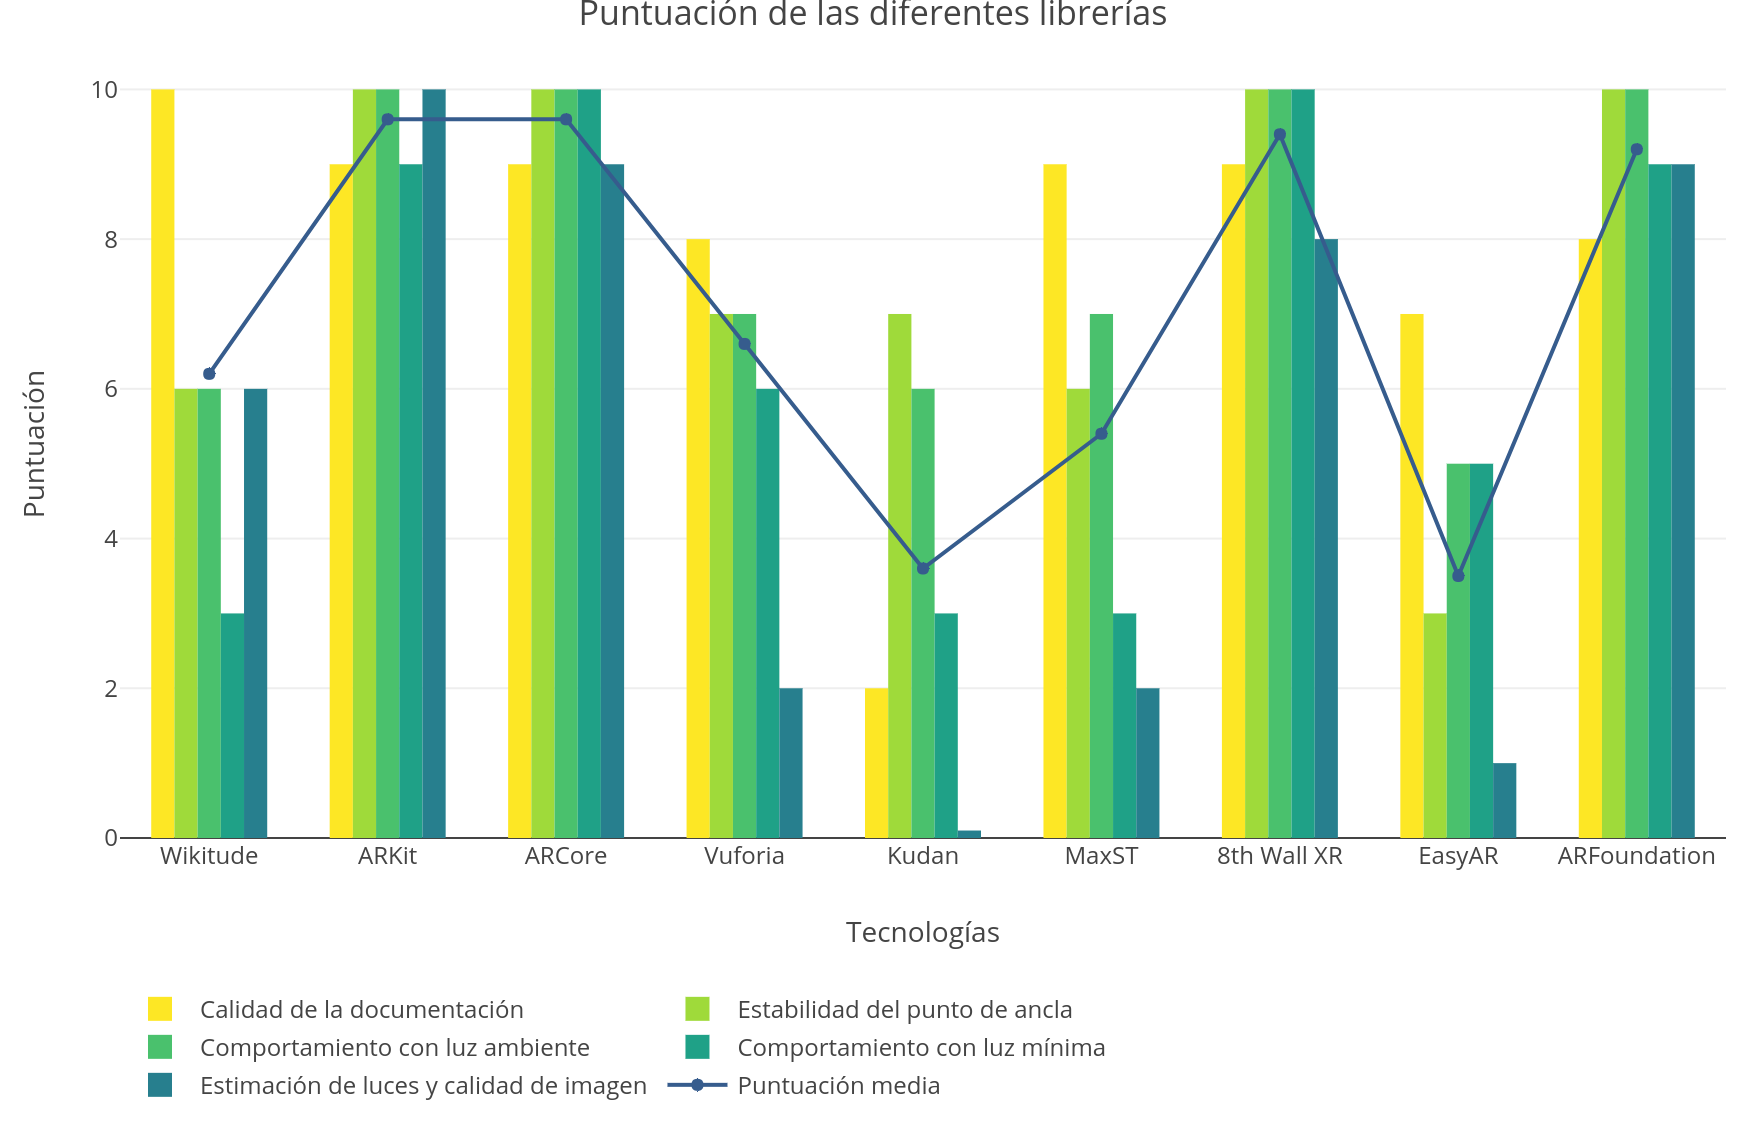
\includegraphics[width=\linewidth]{Images/Puntuacion_librerias.png}
    \caption{Puntuación de las librerías}
    \label{PuntuacionGraph}
\end{figure}

Como se puede observar en la tabla~\ref{PuntuacionGraph}, una vez probadas y comparadas todas las aplicaciones de carácter básico de las librerías, es evidente que ARKit y ARCore son claros ganadores a nivel general, pero entraremos en detalle para ver las funcionalidades y limitaciones de cada una, por lo que vamos a definir nuestra opinión sobre su uso\\

Lo primero que podemos observar es que las librerías que usan detección de planos tienen una precisión y estabilidad increíble, permitiendo un paseo libre por el entorno sin que el ancla presente ningún desplazamiento o cambio de escala. Por el otro lado, tenemos las librerías que utilizan \textit{instant tracking}, aunque su resistencia a movimientos bruscos y a giros sea muy buena en algunos casos, la estabilidad del punto de anclaje cuando nos movemos es bastante pobre.\\

Si queremos realizar una aplicación donde la estabilidad y precisión del ancla sea estricta, lo más seguro es optar por usar la tecnología de detección de planos. Además de la precisión que proporcionan estas librerías, también implementan la estimación de luz, la cual aporta una pincelada de realismo muy importante para la experiencia inmersiva. Las limitaciones de esta tecnología vienen dadas por el entorno, ya sea por el espacio libre que haya para reconocer un plano, por el nivel de luz o por el tipo de superficie. Si la superficie es de color liso, seguramente haya dificultades para reconocer el plano, y finalmente debido al alto coste computacional, la cantidad de dispositivos soportados.\\

Los puntos fuertes de las librerías que utilizan \textit{instant tracking} suplen las limitaciones vistas anteriormente. Su uso es recomendado en aplicaciones pensadas para ser usadas en cualquier entorno, sin depender ni del nivel de luz ni de la superficie que nos rodea, y para cuando no sea necesario moverse en el entorno. Además, cubre un rango muy amplio de dispositivos~\cite{wikitudeInstant}, por lo que se puede llegar a un público mayor. \\

Si miramos la calidad de la experiencia, está claro que usando la detección de planos, como puede ser ARKit y ARCore, obtenemos mejores resultados frente al \textit{instant tracking}, pero no es suficiente para posicionarse como la principal solución para todas las ideas del mercado. Aunque los resultados obtenidos por el \textit{instant tracking} sean peores, sus posibilidades de funcionar en casi cualquier dispositivo, momento y entorno hace que sea una opción a tener en cuenta para muchas aplicaciones.


\noindent